\documentclass[a4paper,12pt]{article}
\usepackage[utf8]{inputenc}
\usepackage{geometry}
\geometry{margin=1in}
\usepackage{graphicx}
\usepackage{caption}
\usepackage{booktabs}
\usepackage{array}
\usepackage{amsmath}
\usepackage{amsfonts}
\usepackage{hyperref}
\usepackage{xcolor}
\usepackage{float}

\title{Part1 :Digit Classification on Reduced MNIST Dataset Using MLP and CNN}

\begin{document}

\maketitle

\section{Introduction}
The Reduced MNIST dataset, a subset of the MNIST dataset, consists of 1000 training examples and 200 testing examples per digit (0-9), with images of size 28x28 pixels in grayscale. This assignment is divided into two parts:

\begin{itemize}
    \item \textbf{Part 1 (MLP with Feature Extraction):} Implement an MLP with 1, 3, or 5 hidden layers, using features extracted via Principal Component Analysis (PCA), Discrete Cosine Transform (DCT), and Autoencoders (AE).
    \item \textbf{Part 2 (CNN with LeNet-5 Variants):} Train a CNN based on the LeNet-5 architecture, adjusting the structure to fit 28x28 images, and explore at least two variations in hyperparameters.
\end{itemize}

The objective is to compare the performance of these models in terms of accuracy, training time, and testing time, and to provide insights into the impact of architectural choices.

\section{Methodology}

\subsection{Dataset}
The Reduced MNIST dataset contains:
\begin{itemize}
    \item \textbf{Training Set:} 1000 examples per digit (10,000 total).
    \item \textbf{Testing Set:} 200 examples per digit (2,000 total).
\end{itemize}
Images are 28x28 pixels in grayscale, and labels correspond to digits 0-9.

\subsection{Part 1: Multi-Layer Perceptron (MLP) with Feature Extraction}
In this part, we implemented an MLP with 1, 2, and 3 hidden layers, using features extracted from the images via three methods:
\begin{itemize}
    \item \textbf{PCA:} Reduced dimensionality while retaining 95\% variance.
    \item \textbf{DCT:} Extracted frequency-based features (225 components).
    \item \textbf{Autoencoder (AE):} Learned a compressed representation (225 components) using an encoder-decoder network.
\end{itemize}
The MLP architectures were trained for 40 epochs with a batch size of 64, using the Adam optimizer.

\subsection{Part 2: Convolutional Neural Network (CNN) with LeNet-5 Variants}
We implemented a CNN based on the LeNet-5 architecture, adjusted for 28x28 images. The base model consists of:
\begin{itemize}
    \item Two convolutional layers (6 and 16 filters, 5x5 kernels, ReLU activation).
    \item Average pooling layers (2x2, stride 2).
    \item Three fully connected layers (120, 84, and 10 units, with ReLU for hidden layers and softmax for output).
\end{itemize}
The model was trained for 40 epochs with a batch size of 64, using the Adam optimizer (except where specified). We explored the following variations:
\begin{itemize}
    \item \textbf{Variation 1 (Increased Filters):} Increased the number of filters to 18 and 24 in the convolutional layers.
    \item \textbf{Variation 2 (Tanh Activation):} Used tanh activation instead of ReLU.
    \item \textbf{Variation 3 (ELU Activation):} Used ELU activation instead of ReLU.
    \item \textbf{Variation 4 (Fewer Layers):} Removed one dense layer (120 units).
    \item \textbf{Variation 5 (Additional Layer):} Added a dense layer (42 units).
    \item \textbf{Variation 6 (MaxPooling):} Replaced AveragePooling with MaxPooling.
    \item \textbf{Variation 7 (Dropout):} Added dropout layers for regularization (0.25 after convolutional layers, 0.5 after the first dense layer).
    \item \textbf{Variation 8 (Batch Normalization):} Added batch normalization after convolutional and dense layers.
    \item \textbf{Variation 9 (SGD Optimizer):} Used SGD with momentum (learning rate 0.01, momentum 0.9) instead of Adam.
    \item \textbf{Variation 10 (Smaller Kernel):} Used 3x3 kernels instead of 5x5.
\end{itemize}

\section{Results}

\subsection{Part 1: MLP with Feature Extraction}
The MLP models were trained with 1, 2, and 3 hidden layers, using features extracted via PCA, DCT, and Autoencoder. The results for each configuration are presented below, along with specific observations and comments.

\begin{figure}[H]
    \centering
    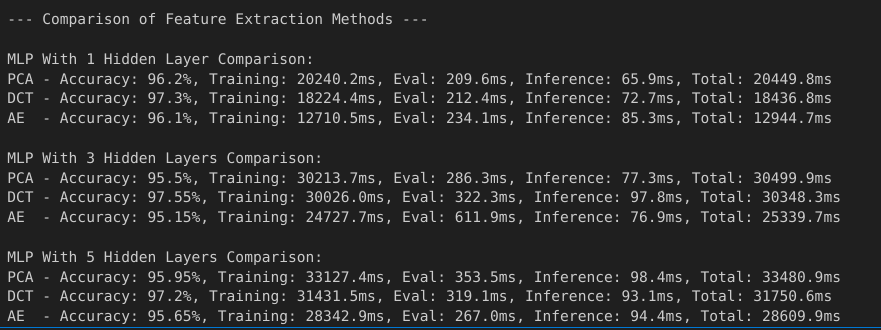
\includegraphics[width=0.8\textwidth]{MLPlayers.png}
    \caption{MLP with 1,3,5 Hidden Layer: Comparison of PCA, DCT, and Autoencoder.}
    \label{fig:mlp_1_hidden}
\end{figure}

\textbf{Observations and Comments for MLP with 1 Hidden Layer:}
\begin{itemize}
    \item \textbf{Accuracy:} DCT achieved the highest accuracy at 97.2\%, followed by PCA at 95.6\%, and Autoencoder at 93.55\%. This suggests that DCT features are particularly effective for simpler MLP architectures, likely due to their ability to capture frequency-based patterns in the data.
    \item \textbf{Training Time:} DCT was the fastest to train (14.8s), compared to PCA (20.3s) and Autoencoder (16.1s). The shorter training time for DCT may be attributed to its efficient feature representation, which reduces the computational burden on the MLP.
    \item \textbf{Inference Time:} Inference times were similar across all methods, with PCA at 65.9ms, Autoencoder at 66.7ms, and DCT at 69.8ms. This indicates that the choice of feature extraction method has a minimal impact on inference speed for a single hidden layer.
    \item \textbf{Comment:} The superior performance of DCT in both accuracy and training time makes it the preferred feature extraction method for a 1-hidden-layer MLP. Autoencoder's lower accuracy suggests that the learned features may not be as discriminative for this task.
\end{itemize}

\textbf{Observations and Comments for MLP with 2 Hidden Layers:}
\begin{itemize}
    \item \textbf{Accuracy:} DCT again outperformed the others with an accuracy of 97.35\%, slightly better than its 1-hidden-layer performance. PCA achieved 95.55\%, nearly identical to its 1-hidden-layer result, while Autoencoder improved slightly to 93.8\%. The marginal improvement in DCT's accuracy suggests that adding a second hidden layer enhances its ability to model complex patterns in the frequency domain.
    \item \textbf{Training Time:} Training times increased for all methods due to the additional layer: DCT took 22.4s, PCA 28.0s, and Autoencoder 24.4s. PCA's training time increased the most, indicating that its features may require more computation to process through deeper networks.
    \item \textbf{Inference Time:} Inference times also increased slightly, with DCT at 71.8ms, PCA at 68.0ms, and Autoencoder at 71.1ms. The increase is expected due to the additional layer, but the differences remain small.
    \item \textbf{Comment:} The 2-hidden-layer MLP with DCT features strikes a good balance between accuracy and training time, achieving the highest accuracy across all MLP configurations. The slight improvement in Autoencoder's accuracy suggests that deeper architectures may help it capture more relevant features, but it still lags behind DCT and PCA.
\end{itemize}

\textbf{Observations and Comments for MLP with 3 Hidden Layers:}
\begin{itemize}
    \item \textbf{Accuracy:} DCT maintained a high accuracy of 97.0\%, but it decreased slightly from the 2-hidden-layer configuration (97.35\%). PCA's accuracy dropped significantly to 93.35\%, and Autoencoder's accuracy was the lowest at 93.2\%. This decline in accuracy for PCA and Autoencoder suggests potential overfitting or loss of generalization as the model becomes deeper.
    \item \textbf{Training Time:} Training times were the highest for this configuration, with DCT at 26.9s, PCA at 28.3s, and Autoencoder at 27.1s. The similar training times across methods indicate that the computational cost of adding a third hidden layer is consistent regardless of the feature type.
    \item \textbf{Inference Time:} Inference times increased further, with DCT at 83.4ms, PCA at 79.7ms, and Autoencoder at 81.5ms. DCT's inference time increased the most, likely due to the complexity of processing its features through three hidden layers.
    \item \textbf{Comment:} The 3-hidden-layer MLP shows diminishing returns in accuracy for all feature types, with DCT being the only method to maintain a high accuracy (97.0\%). The significant drop in PCA and Autoencoder performance suggests that deeper MLPs may not be suitable for these features on the Reduced MNIST dataset, as they may overfit or fail to generalize effectively.
\end{itemize}

\subsection{Part 2: CNN with LeNet-5 Variants}
The CNN models were trained with the base LeNet-5 architecture and 10 variations. The results are summarized below, with screenshots of the output for each variant.

\begin{figure}[H]
    \centering
    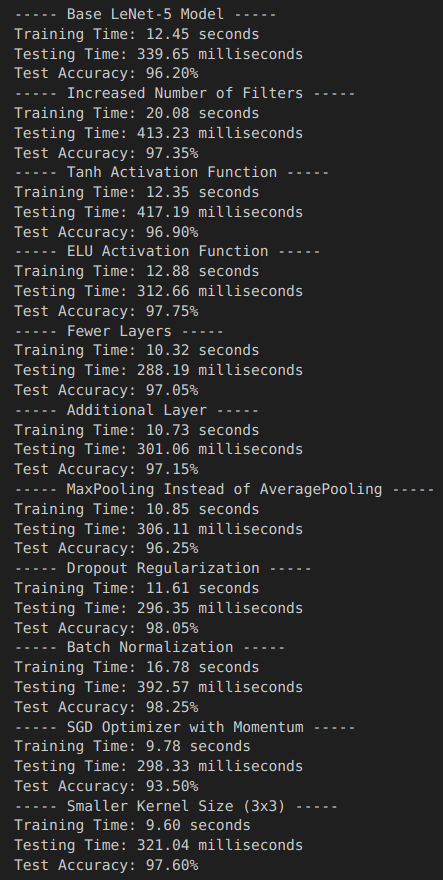
\includegraphics[width=0.8\textwidth]{CNNvariations.png}
    \caption{Base LeNet-5 Model Results vs Variations.}
    \label{fig:cnn_base}
\end{figure}


\textbf{Observations on Variations:}
\begin{itemize}
    \item \textbf{Accuracy Trends:} The highest accuracy was achieved with batch normalization (98.25\%), followed closely by dropout regularization (98.05\%). This suggests that regularization techniques are crucial for improving generalization on the Reduced MNIST dataset. The lowest accuracy was observed with the SGD optimizer (93.50\%), indicating that adaptive optimizers like Adam are more effective for this task.
    \item \textbf{Impact of Activation Functions:} ELU activation (97.75\%) outperformed both ReLU (base model, 96.20\%) and tanh (96.90\%), likely due to its ability to handle negative inputs and improve gradient flow, leading to better convergence.
    \item \textbf{Effect of Layer Modifications:} Removing a dense layer (Variation 4) reduced training time to 10.32s while maintaining a high accuracy (97.05\%), suggesting that a simpler architecture can be effective for this dataset. Conversely, adding a dense layer (Variation 5) slightly improved accuracy (97.15\%) but increased training time marginally (10.73s).
    \item \textbf{Pooling Methods:} MaxPooling (96.25\%) performed worse than AveragePooling (base model, 96.20\%), possibly because MaxPooling discards more spatial information, which may be critical for small 28x28 images.
    \item \textbf{Regularization Benefits:} Both dropout (98.05\%) and batch normalization (98.25\%) significantly improved accuracy over the base model, with batch normalization providing the best performance. However, batch normalization increased training time (16.78s) due to additional computations.
    \item \textbf{Optimizer Performance:} The SGD optimizer with momentum resulted in the lowest accuracy (93.50\%) but the fastest training time (9.78s), highlighting the trade-off between optimization efficiency and model performance.
    \item \textbf{Kernel Size Impact:} Using a smaller 3x3 kernel (97.60\%) achieved a high accuracy with the fastest training time (9.60s), indicating that smaller kernels can effectively capture features in this dataset while reducing computational complexity.
    \item \textbf{Training and Testing Time Variations:} Training time varied significantly, with the increased filters model being the slowest (20.08s) due to higher computational complexity, and the smaller kernel model being the fastest (9.60s). Testing time (inference time for the entire test set) ranged from 288.19ms (fewer layers) to 417.19ms (tanh activation), showing that architectural choices impact inference speed.
\end{itemize}
\newpage
\section{Comparison of MLP and CNN Results}
The table below compares the results of the MLP models (Part 1) and CNN models (Part 2) from Assignment 2. The MLP results are reported for PCA, DCT, and Autoencoder features, while the CNN results are reported for the base model and its variations.

\begin{table}[H]
    \centering
    \caption{Comparison of Classification Performance for MLP and CNN Models}
    \label{tab:comparison}
    \resizebox{\textwidth}{!}{
    \begin{tabular}{l|cc|cc|cc}
        \toprule
        \multirow{2}{*}{\textbf{Classifier}} & \multicolumn{2}{c|}{\textbf{DCT}} & \multicolumn{2}{c|}{\textbf{PCA}} & \multicolumn{2}{c}{\textbf{Autoencoder}} \\
        \cmidrule(lr){2-3} \cmidrule(lr){4-5} \cmidrule(lr){6-7}
        & \textbf{Accuracy (\%)} & \textbf{Processing Time (ms)} & \textbf{Accuracy (\%)} & \textbf{Processing Time (ms)} & \textbf{Accuracy (\%)} & \textbf{Processing Time (ms)} \\
        \midrule
        \multicolumn{7}{c}{\textbf{DCT and PCA features from Assignment 1}} \\
        \midrule
        \multirow{K-means Clustering} & - & - & - & - & - & - \\
        1 & 86.85 & & 86.8 & & - & - \\
        4 & 92.25 & & 92.1 & & - & - \\
        16 & 94.4 & & 94.6 & & - & - \\
        32 & 95.9 & & 95.8 & & - & - \\
        \midrule
        \multirow{SVM} & - & - & - & - & - & - \\
        Linear & 94.4 & & 93.85 & & - & - \\
        Nonlinear & 97.1 & & 97.65 & & - & - \\
        \midrule
        \multicolumn{7}{c}{\textbf{Multi-layer Perceptron (MLP) - Assignment 2}} \\
        \midrule
        \textbf{Variations} & \multicolumn{2}{c|}{\textbf{DCT}} & \multicolumn{2}{c|}{\textbf{PCA}} & \multicolumn{2}{c}{\textbf{Autoencoder}} \\
        \cmidrule(lr){2-3} \cmidrule(lr){4-5} \cmidrule(lr){6-7}
        1-Hidden & 97.3 & 68.6 & 95.85 & 67.3 & 93.65 & 72.8 \\
        3-Hidden & 97.15 & 75,2 & 94 & 75.2 & 93.4 & 79.5 \\
        5-Hidden & 97.2 & 79.1 & 95.6 & 82.6 & 93 & 85.6 \\
        \midrule
        \multicolumn{7}{c}{\textbf{In the CNN Model no Features are needed - Assignment 2}} \\
        \midrule
        \textbf{Variations} & \multicolumn{2}{c}{\textbf{Accuracy (\%)}} & \multicolumn{2}{c}{\textbf{Training Time (ms)}} & \multicolumn{2}{c}{\textbf{Testing Time (ms)}} \\
        \cmidrule(lr){2-3} \cmidrule(lr){4-5} \cmidrule(lr){6-7}
        Base LeNet-5 & \multicolumn{2}{c}{96.20} & \multicolumn{2}{c}{12450} & \multicolumn{2}{c}{339.65} \\
        Variation 1: Increased Filters & \multicolumn{2}{c}{97.35} & \multicolumn{2}{c}{20080} & \multicolumn{2}{c}{413.23} \\
        Variation 2: Tanh Activation & \multicolumn{2}{c}{96.90} & \multicolumn{2}{c}{12350} & \multicolumn{2}{c}{417.19} \\
        Variation 3: ELU Activation & \multicolumn{2}{c}{97.75} & \multicolumn{2}{c}{12880} & \multicolumn{2}{c}{312.66} \\
        Variation 4: Fewer Layers & \multicolumn{2}{c}{97.05} & \multicolumn{2}{c}{10320} & \multicolumn{2}{c}{288.19} \\
        Variation 5: Additional Layer & \multicolumn{2}{c}{97.15} & \multicolumn{2}{c}{10730} & \multicolumn{2}{c}{301.06} \\
        Variation 6: MaxPooling & \multicolumn{2}{c}{96.25} & \multicolumn{2}{c}{10850} & \multicolumn{2}{c}{306.11} \\
        Variation 7: Dropout & \multicolumn{2}{c}{98.05} & \multicolumn{2}{c}{11610} & \multicolumn{2}{c}{296.35} \\
        Variation 8: Batch Normalization & \multicolumn{2}{c}{98.25} & \multicolumn{2}{c}{16780} & \multicolumn{2}{c}{392.57} \\
        Variation 9: SGD Optimizer & \multicolumn{2}{c}{93.50} & \multicolumn{2}{c}{9780} & \multicolumn{2}{c}{298.33} \\
        Variation 10: Smaller Kernel & \multicolumn{2}{c}{97.60} & \multicolumn{2}{c}{9600} & \multicolumn{2}{c}{321.04} \\
        \bottomrule
    \end{tabular}
    }
\end{table}
\section{Discussion}
The CNN models generally outperformed the MLP models in terms of accuracy, with the best CNN variant (Batch Normalization, 98.25\%) surpassing the best MLP configuration (DCT with 2 hidden layers, 97.35\%). This is expected, as CNNs are designed to capture spatial hierarchies in image data directly, whereas MLPs rely on pre-extracted features, which may not fully represent the data's spatial structure.\\
For the MLP models, DCT features consistently provided the highest accuracy (up to 97.35\% with 2 hidden layers), suggesting that frequency-based features are particularly effective for digit classification. However, the performance of PCA and Autoencoder features degraded with deeper architectures (e.g., PCA accuracy dropped from 95.6\% to 93.35\% as hidden layers increased from 1 to 3), indicating that deeper MLPs may overfit or fail to generalize well with these features. Additionally, the inference time for MLPs was significantly lower (e.g., 69.8ms for DCT with 1 hidden layer) compared to CNNs (e.g., 413.23ms for the increased filters variant), making MLPs more suitable for applications requiring fast inference.\\
Among the CNN variants, regularization techniques (dropout and batch normalization) yielded the highest accuracies (98.05\% and 98.25\%, respectively), highlighting the importance of preventing overfitting on the Reduced MNIST dataset. The ELU activation function (97.75\%) also improved performance over ReLU (96.20\%) and tanh (96.90\%), likely due to its ability to mitigate vanishing gradient issues and handle negative inputs effectively. Conversely, the SGD optimizer performed poorly (93.50\%), suggesting that adaptive optimizers like Adam are better suited for this task.\\
Training time varied significantly across CNN variants, with the increased filters model being the slowest (20.08s) due to the higher number of parameters, and the smaller kernel model being the fastest (9.60s) due to reduced computational complexity. Testing time (inference time for the entire test set) was lowest for the fewer layers variant (288.19ms) and highest for the tanh activation variant (417.19ms), indicating that architectural choices impact not only training but also inference efficiency.\\
Interestingly, simpler CNN architectures (e.g., fewer layers, smaller kernels) achieved competitive accuracies (97.05\% and 97.60\%, respectively) with significantly reduced training times (10.32s and 9.60s), suggesting that the Reduced MNIST dataset does not require overly complex models to achieve high performance. This balance between accuracy and efficiency is crucial for practical applications where computational resources are limited.

\section{Conclusion}
This study demonstrates that CNNs, particularly with regularization techniques like batch normalization (98.25\%) and dropout (98.05\%), achieve superior accuracy on the Reduced MNIST dataset compared to MLPs with feature extraction (best at 97.35\% with DCT). The CNN's ability to directly process raw images and capture spatial features makes it more effective for this task, although MLPs with DCT features offer a competitive alternative with faster inference times (e.g., 69.8ms vs. 392.57ms for the best CNN).\\
Among the CNN variants, batch normalization and dropout provided the best performance, while simpler architectures (e.g., smaller kernels, fewer layers) achieved a good balance between accuracy and computational efficiency. For the MLP models, DCT features were the most effective, but deeper architectures led to diminished returns in accuracy, suggesting that simpler models may be preferable for this dataset.\\
Future work could explore hybrid approaches, such as using DCT features as input to a CNN, to combine the strengths of both methods. Additionally, experimenting with other regularization techniques (e.g., weight decay) or advanced optimizers (e.g., AdamW) could further improve performance while maintaining efficiency.

\end{document}